\section{Sequential composition with M/M/1/K queues}
    \paragraph{Why M/M/1/K queues?} An average component in a distributed system can be modeled as an M/M/1/K, due to the exponential inter-arrival rate of messages, the exponential distribution of the execution delay and the message buffer size of a component.
    
    \subsection{System composition}
    The system has two components \texttt{worker\_1}, \texttt{worker\_2}, the components are made of a buffer queue of size $K$ and a worker process.
    
    The system sends $n$ messages per second following a Poisson distribution to \texttt{worker\_1}'s queue, the queue then reduces its available buffer size. \\
    
    The buffer notifies its worker, which then does $N$ loops, which are defined upon start, of fictional work. The worker then passes a message to \texttt{worker\_2}'s queue, which has another queue of same size, who passes the message to \texttt{worker\_2}'s worker, which does the same amount of loops. When a worker completes its work, it notifies the queue, freeing one "message" from its buffer size. \\
    
    If the queue's buffer is overloaded, it will drop the incoming message and consider the execution a failure. \\
    
    A probe $p$ is defined, which observes the execution from when the first message up until \texttt{worker\_2} is done.
    \begin{figure}[H]
        \begin{center}
            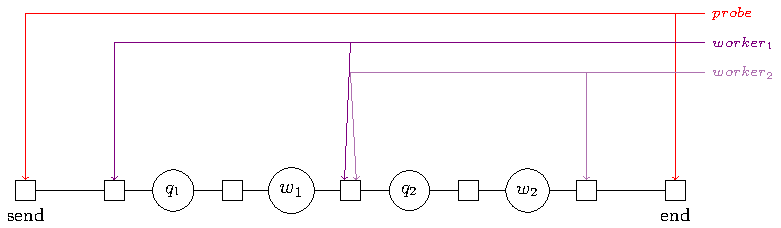
\includegraphics[scale=1.2, width=\textwidth]{tikz/mm1k.pdf} 
        \end{center}
        \caption{Outcome diagram of the M/M/1/K queue with the colored lines representing the probes that were inserted.}
        \label{fig:mm1k}
    \end{figure}

    \subsection{Determining parameters dynamically}
        We stated previously that determining parameters is something that must be done with an underlying knowledge of the system. The oscilloscope can provide knowledge of the system, here is an example of worker\_1 and worker\_2 as observed in the oscilloscope.

        Imagine the engineer supposes the workers executions should take around 6.5 ms to complete, but doesn't actually know how long the executions should take. The engineer, after having set the required parameters observes in the following graph in the oscilloscope \cref{fig:w1w2}.

    The oscilloscope shows the engineer that their assumptions do not correspond to the actual system $\Delta$Q, the user can then modify the parameters to observe the actual system's behaviour. By setting $dmax$ to 25 ms, he can observe the worker's $\Delta$Qs approaching 1.

\begin{figure}[H]
            \centering
            \begin{subfigure}{.5\textwidth}
                \centering
                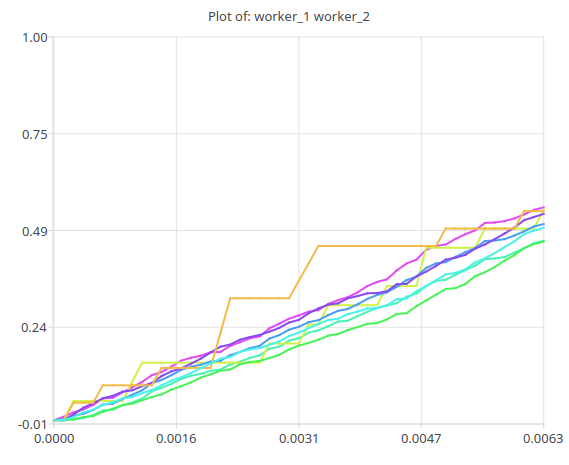
\includegraphics[width=0.98\textwidth]{img/w1w2.png}
                \label{fig:w1w2}
                \subcaption{worker\_1 and worker\_2 $\Delta$Qs plot with 6.5 ms $dMax$.}
            \end{subfigure}%
            \begin{subfigure}{.5\textwidth}
                \centering
                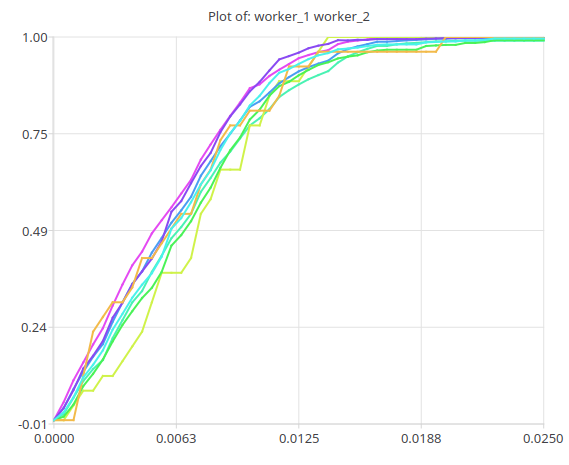
\includegraphics[width =0.98\textwidth]{img/w1w2hb.png}
                \label{fig:sub2}
                \subcaption{worker\_1 and worker\_2 $\Delta$Qs plot with 25 ms $dMax$} 
            \end{subfigure}
            \label{fig:w1w2hb}
            \end{figure}


    On the other hand, the engineer's assumption could have been what he truly expected from the system, in this case, the oscilloscope tells him that the system is not behaving as expected. 

    \paragraph{Low Load}

    At low load, we can observe in the oscilloscope how worker\_1 and worker\_2 mean $\Delta$Qs overlap. This is expected, even under overload or dependency conditions, worker\_1 and worker\_2 should have the same $\Delta$Qs.

If the system is not showing dependent behaviour, the probe \textbf{observed $\Delta$Q} and \textbf{calculated $\Delta$Q} should overlap. We can observe that in the graph below, as the mean CDF of both $\Delta$Qs overlap.



\begin{figure}[H]
            \centering
            \begin{subfigure}{.5\textwidth}
                \centering
                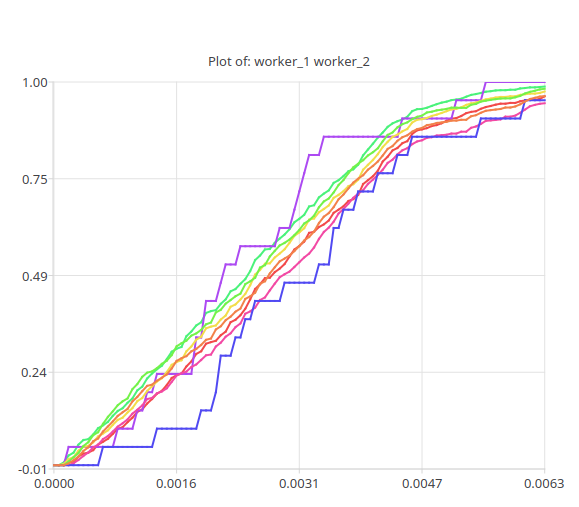
\includegraphics[width=0.98\textwidth]{img/superp21.png}
                \label{fig:sp21}
                \subcaption{worker\_1 (blue) and worker\_2 (purple) $\Delta$Q plots as shown in the oscilloscope}
            \end{subfigure}%
            \begin{subfigure}{.5\textwidth}
                \centering
                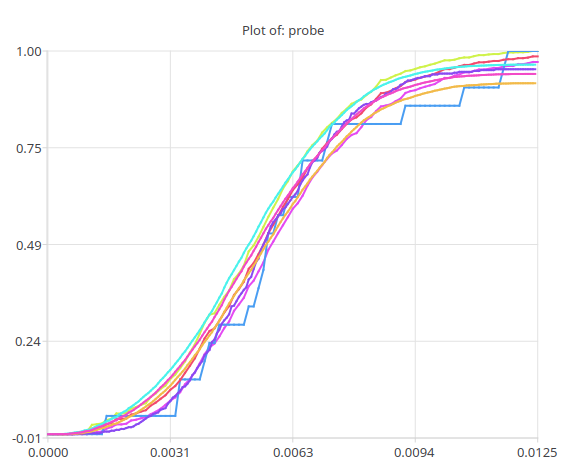
\includegraphics[width =0.98\textwidth]{img/superp22.png}
                \label{fig:sub2}
                \subcaption{probe $\Delta$Q plots as shown in the oscilloscope} 
            \end{subfigure}
            \label{fig:sp22}
            \end{figure}

\paragraph{Early signs of overload}
    
    Once the system is approaching overload, we can see the two means starting to diverge. As shown in a previous chapter, the observed (1) $\Delta$Q of the probe is below the calculated (2) $\Delta$Q. (explain better) 
    \begin{figure}[H]
        \begin{center}
            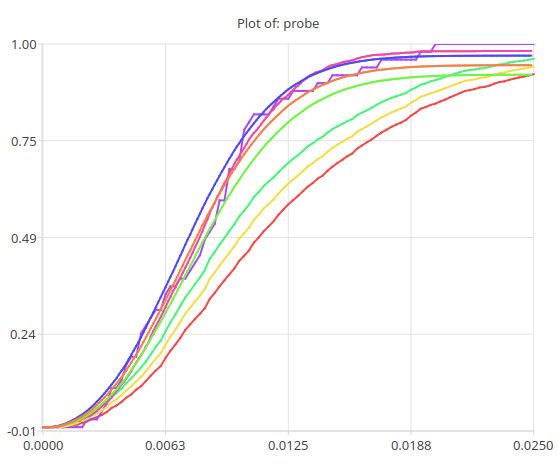
\includegraphics[scale=0.6]{img/diverging11.png}
        \end{center}
    \end{figure}

    \subsection{Triggers - QTA}
        Triggers and QTAs are an important part of the oscilloscope and $\Delta$QSD, we will show here how they can be used and what $\Delta$Q can tell about the state of the system.

        \paragraph{Satisfying timeliness, a tale of typical queue behaviour}

        $\Delta$Q can be used to feel overload approaching and analyse a system's behaviour. To do so, we set a QTA for the probe. 25\% of instances should take $< 6.5$ ms, 50\% $<12 ms$, 75\% $<17 ms$. We run the program and wait for triggers to be fired. To do so, we synthetically overload the CPU to degrade the system's performance.
         
        \begin{wrapfigure}{R}{0.3\textwidth}
            \caption{The snapshots fired during execution, we will select the snapshot triggered at 17:52:33}\label{wrap-fig:1}
            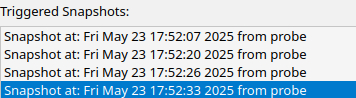
\includegraphics[width=0.25\textwidth]{img/snapshots.png}
        \end{wrapfigure} 

        From the $\Delta$Qs we have in the snapshot we can observe:
        \begin{enumerate}
            \item \textbf{Business as usual}: The system is not showing signs of stress, the $\Delta$Q is better than or between than the confidence bounds.
            \item \textbf{Overload approaching}: The component is slowing down and the $\Delta$Q is  slightly worse than previously, but we can still feel overload is approaching.
            \item \textbf{QTA violation}: The queue, overloaded, quickly violates the QTA.
            \item \textbf{Get in trouble quickly, get out of it slowly}: The buffering filling up quickly and emptying slowly is a typical queue pattern, this can be observed on the oscilloscope
        \end{enumerate}
        
        For the following graphs, the \textbf{blue} line, annotated as \textbf{(1)} is the \textbf{observed $\Delta$Q}, the \textbf{red} line, annotated as \textbf{(2)}, is the \textbf{calculated $\Delta$Q}. 
        \subsubsection{Business as usual}
            During normal execution, we can observe the system behaving correctly for a long time before the trigger is fired. This is what the user who connects the oscilloscope to a system which correctly behaves should see most of the time.
        \begin{figure}[H]
            \centering
            \begin{subfigure}{.5\textwidth}
                \centering
                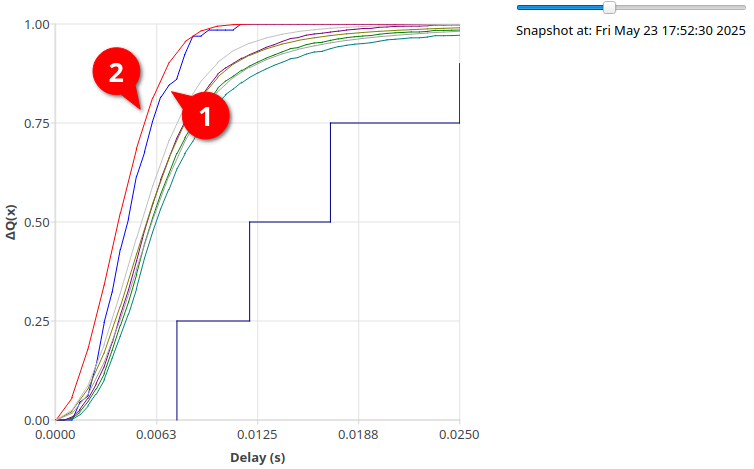
\includegraphics[width=0.98\textwidth]{img/norm_ex_32.png}
                \label{fig:norm_ex_1}
            \end{subfigure}%
            \begin{subfigure}{.5\textwidth}
                \centering
                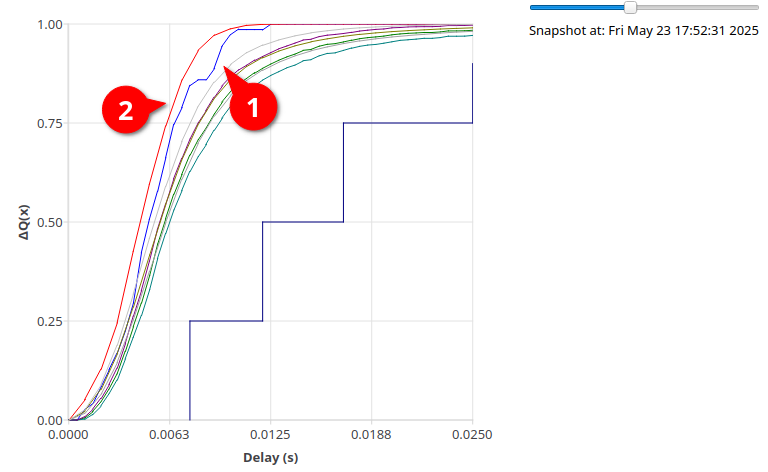
\includegraphics[width =0.98\textwidth]{img/normal.png}
                \label{fig:norm_ex_2}
            \end{subfigure}
            \label{fig:norm_ex}
            \caption{Normal execution of the system over 2 seconds before overload.}
            \end{figure}
        
        \subsubsection{Overload approaching}
            We can remark the system approaching overload just before the system violates the QTA. While no triggers are yet fired, as the system is still respecting QTA, we canfeel something is starting to go wrong.
        \begin{figure}[H]
            \centering
            \begin{subfigure}{.5\textwidth}
                \centering
                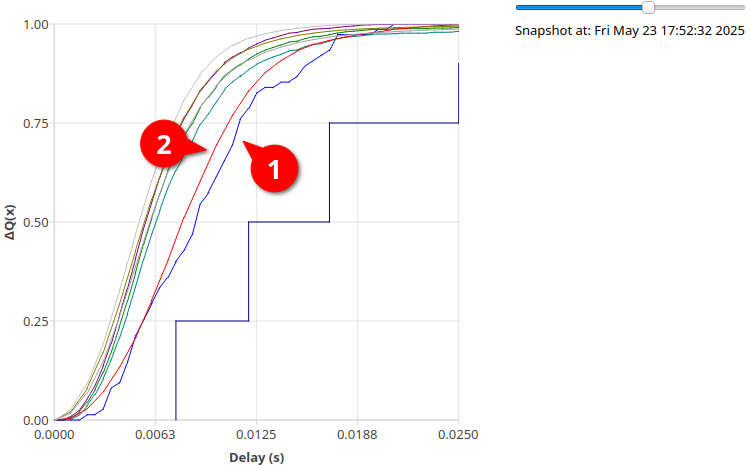
\includegraphics[width=0.98\textwidth]{img/early_sign2.png}
                \label{fig:appr_ov_2}
            \end{subfigure}%
            \begin{subfigure}{.5\textwidth}
                \centering
                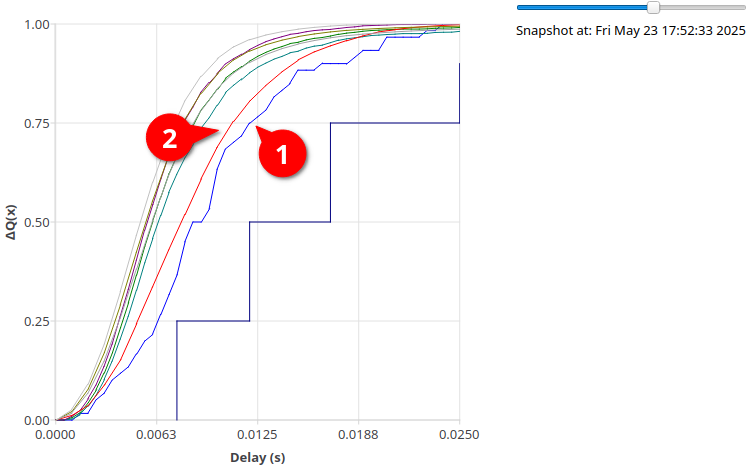
\includegraphics[width =0.98\textwidth]{img/approaching_2.png}
                \label{fig:appr_ov}
            \end{subfigure}
            \label{fig:appr_ov_t}
            \caption{The system is slowly degrading just seconds before overload.}
            \end{figure}
        
        \subsubsection{QTA violation}
            Just moments after the system performance degrading, the observed $\Delta$Q violates the QTA. We point in blue where the violations happen.

            We can observe how the system $\Delta$Q is dangerously close to the QTA bounds right after violating the QTA. This is because the queue will fill up quickly and empty slowly. We can observe in the next section how the repercussions of such violations linger on for some time after the violation happens.
            \begin{figure}[H]
            \centering
            \begin{subfigure}{.5\textwidth}
                \centering
                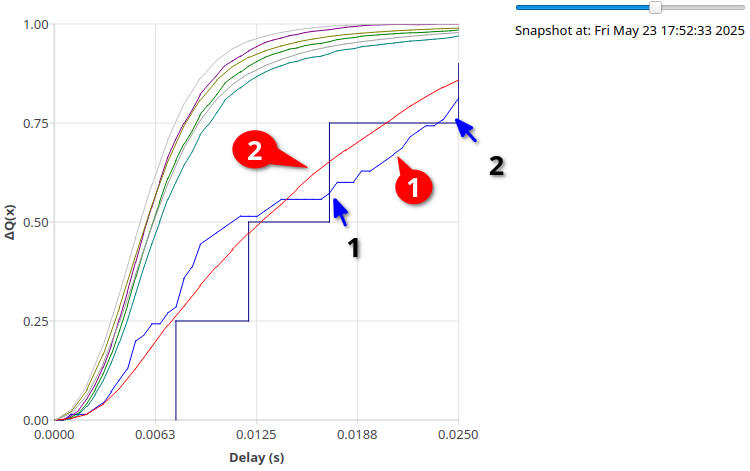
\includegraphics[width=0.98\textwidth]{img/violation1.png}
                \label{fig:violat_1}
            \end{subfigure}%
            \begin{subfigure}{.5\textwidth}
                \centering
                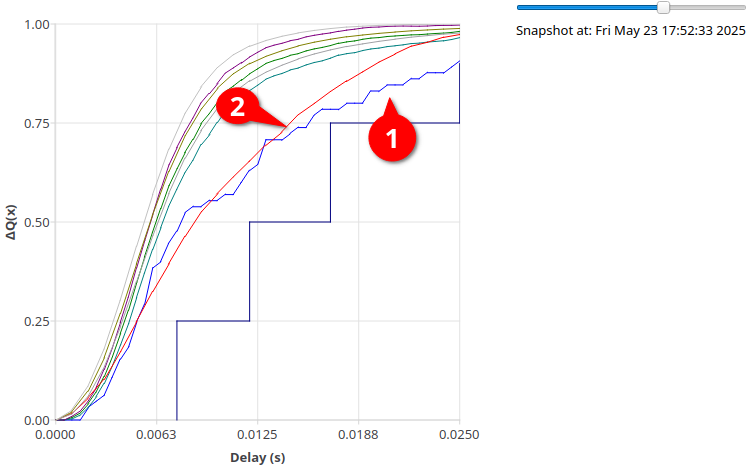
\includegraphics[width =0.98\textwidth]{img/right_after1.png}
                \label{fig:violat_2}
            \end{subfigure}
            \label{fig:violat}
                \caption{Left: The system violates the QTA. Right: The system is slowly recuperating from overload.}
            \end{figure}
 

        \subsubsection{Get in trouble quickly, get out of it slowly}
            By recording a snapshot the system \textbf{after} the violation happens, we can observe how long it takes to get out. 
        \begin{figure}[H]
            \centering
            \begin{subfigure}{.5\textwidth}
                \centering
                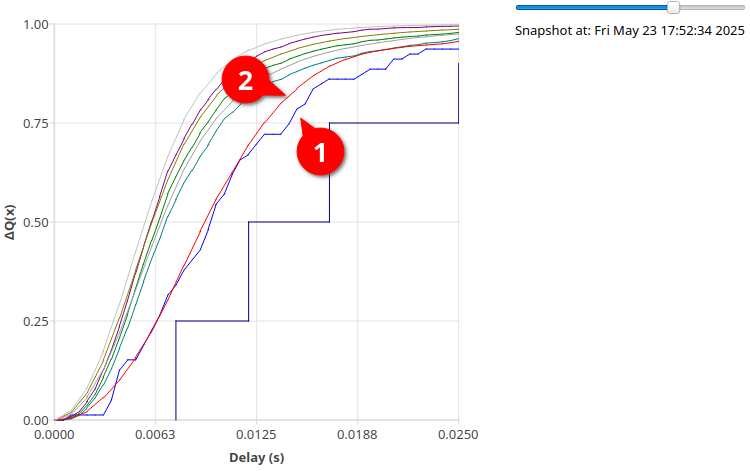
\includegraphics[width=0.98\textwidth]{img/getting_bacl1.png}
                \label{fig:recup_1}
            \end{subfigure}%
            \begin{subfigure}{.5\textwidth}
                \centering
                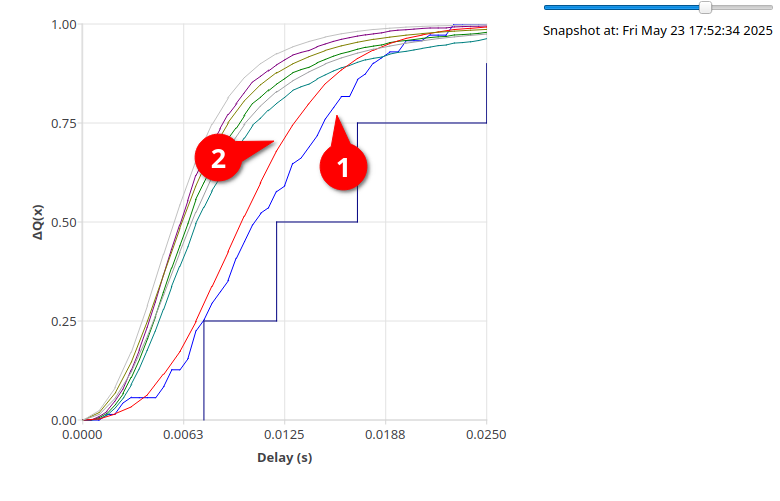
\includegraphics[width =0.98\textwidth]{img/still_bad12.png}
                \label{fig:recup_2}
            \end{subfigure}
            \label{fig:recup}
            \caption{The system is slowly degrading just seconds before overload.}
            \end{figure}
            
            The system gets out of dangerous grounds \textbf{2 seconds} after violating the QTA, and still shows the consequences of overload 3 seconds after.

        \begin{figure}[H]
            \centering
            \begin{subfigure}{.5\textwidth}
                \centering
                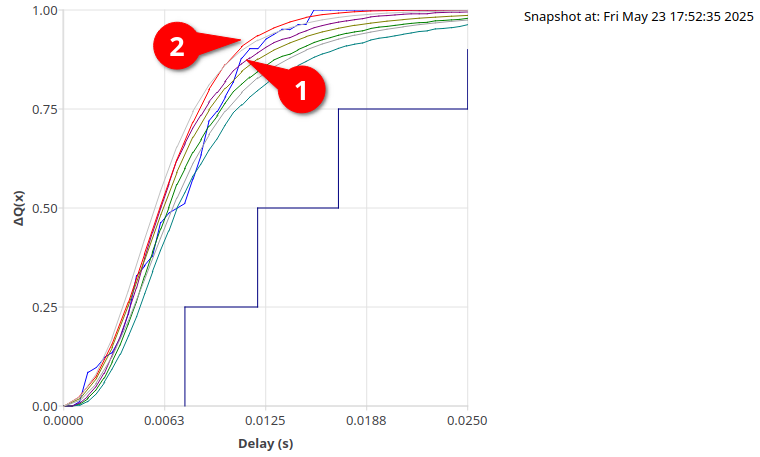
\includegraphics[width=0.98\textwidth]{img/return_2g1.png}
                \label{fig:appr_ov_2}
            \end{subfigure}%     
        \end{figure}%
    
